%----------------------------------------------------------------------------------------
%	PACKAGES AND OTHER DOCUMENT CONFIGURATIONS
%----------------------------------------------------------------------------------------

\documentclass[paper=a4, fontsize=10pt]{scrartcl} % A4 paper and 10pt font size

\usepackage[T1]{fontenc} % Use 8-bit encoding that has 256 glyphs
%\usepackage{fourier} % Use the Adobe Utopia font for the document - comment this line to return to the LaTeX default
\usepackage[english]{babel} % English language/hyphenation
\usepackage{amsmath,amsfonts,amsthm} % Math packages
\usepackage{algorithm}
%\usepackage{algorithmic}
\usepackage{algpseudocode}
\renewcommand{\algorithmicrequire}{\textbf{Input:}} % Use Input in the format of Algorithm
\renewcommand{\algorithmicensure}{\textbf{Output:}} % Use Output in the format of Algorithm
\usepackage{color}
\usepackage[colorlinks, linkcolor=black]{hyperref}
\usepackage{graphicx}
\usepackage{subfigure}
\usepackage{color}


\usepackage{geometry}
\geometry{scale=0.8}

 \usepackage{setspace}



\usepackage{lipsum} % Used for inserting dummy 'Lorem ipsum' text into the template

\usepackage{sectsty} % Allows customizing section commands
%\allsectionsfont{\centering \normalfont\scshape} % Make all sections centered, the default font and small caps

\usepackage{fancyhdr} % Custom headers and footers
\pagestyle{fancyplain} % Makes all pages in the document conform to the custom headers and footers
\fancyhead{} % No page header - if you want one, create it in the same way as the footers below
\fancyfoot[L]{} % Empty left footer
\fancyfoot[C]{} % Empty center footer
\fancyfoot[R]{\thepage} % Page numbering for right footer
\renewcommand{\headrulewidth}{0pt} % Remove header underlines
\renewcommand{\footrulewidth}{0pt} % Remove footer underlines
\setlength{\headheight}{0pt} % Customize the height of the header

\numberwithin{equation}{section} % Number equations within sections (i.e. 1.1, 1.2, 2.1, 2.2 instead of 1, 2, 3, 4)
\numberwithin{figure}{section} % Number figures within sections (i.e. 1.1, 1.2, 2.1, 2.2 instead of 1, 2, 3, 4)
\numberwithin{table}{section} % Number tables within sections (i.e. 1.1, 1.2, 2.1, 2.2 instead of 1, 2, 3, 4)

%\setlength\parindent{0pt} % Removes all indentation from paragraphs - comment this line for an assignment with lots of text

%----------------------------------------------------------------------------------------
%	TITLE SECTION
%----------------------------------------------------------------------------------------

\newcommand{\horrule}[1]{\rule{\linewidth}{#1}} % Create horizontal rule command with 1 argument of height

\title{	
\normalfont \normalsize 
\textsc{Fudan University, Artificial Intelligence} \\ [0pt] % Your university, school and/or department name(s)
\horrule{1pt} \\[0.4cm] % Thin top horizontal rule
\LARGE Report on Project 3: Black Jack \\ % The assignment title
\horrule{1pt} \\[0cm] % Thick bottom horizontal rule
}

\author{Ao Wang, 15300240004} % Your name

\date{\normalsize\today} % Today's date or a custom date

\begin{document}

\begin{spacing}{1.}

\maketitle % Print the title

%----------------------------------------------------------------------------------------
\section{Overview}
This project is about solving Black Jack using MDPs. This pdf contains the answers of the required questions.

\section{Problem 1}
\subsection{Problem 1a}
As required by the instructions, the state -2 and 2 are the exits, so I manually set the $V_{opt}(s)$ of them to a fixed number, which is 0. Then the results are as follows:
\begin{table}[h]
\setlength{\abovecaptionskip}{0.cm}
\setlength{\belowcaptionskip}{-0.cm}
\centering
  \caption{The result of 1st value iteration (after 0 iterations).}
  %\label{tab:test}
  \begin{tabular}{|c|c|c|c|c|c|}
     \hline
    State $s$ & -2 & -1 & 0 & 1 & 2\\
     \hline
    $V_{opt}(s)$ & 0.0 & \textbf{11.0} & \textbf{-5.0} & \textbf{25.0} & 0.0\\
     \hline
  \end{tabular}
\end{table}

\begin{table}[h]
\setlength{\abovecaptionskip}{0.cm}
\setlength{\belowcaptionskip}{-0.cm}
\centering
  \caption{The result of 2nd value iteration (after 1 iterations).}
  %\label{tab:test}
  \begin{tabular}{|c|c|c|c|c|c|}
     \hline
    State $s$ & -2 & -1 & 0 & 1 & 2\\
     \hline
    $V_{opt}(s)$ & 0.0 & \textbf{10.0} & \textbf{10.2} & \textbf{21.5} & 0.0\\
     \hline
  \end{tabular}
\end{table}

\begin{table}[h]
\setlength{\abovecaptionskip}{0.cm}
\setlength{\belowcaptionskip}{-0.cm}
\centering
  \caption{The result of 3rd value iteration (after 2 iterations).}
  %\label{tab:test}
  \begin{tabular}{|c|c|c|c|c|c|}
     \hline
    State $s$ & -2 & -1 & 0 & 1 & 2\\
     \hline
    $V_{opt}(s)$ & 0.0 & \textbf{13.04} & \textbf{8.45} & \textbf{32.14} & 0.0\\
     \hline
  \end{tabular}
\end{table}

\subsection{Problem 1b}
After the iteration is converged, the result of $\pi_{opt}$ is as follows:
\begin{table}[!htbp]
\setlength{\abovecaptionskip}{0.cm}
\setlength{\belowcaptionskip}{-0.cm}
\centering
  \caption{The result of the optimal actions after being converged.}
  %\label{tab:test}
  \begin{tabular}{|c|c|c|c|c|c|}
     \hline
    State $s$ & -2 & -1 & 0 & 1 & 2\\
     \hline
    $\pi_{opt}(s)$ & - & \textbf{-1} & \textbf{+1} & \textbf{+1} & -\\
     \hline
  \end{tabular}
\end{table}

The result is pretty clear because the agent tries to get to the exit as soon as possible as the reward of each step is negative and both of the exits have comparatively high positive rewards. But at state 0, agent will have higher expectation by moving +1, although it has a high possibility of moving -1. The details are in the \texttt{submission.py}.

\section{Problem 2}
\subsection{Problem 2a}
According to the instruction, the transition (probability) has been changed with noise, with a probability to randomly change to a possible reachable state. I can find a counter example that $V_{1}(s_{start}) \le V_{2}(s_{start})$. 

I construct a MDP with three states: -1, 0 and 1. -1 is the exit state with a reward of -20, but 0 and 1 have positive rewards of 10 and 20. In the original MDP, state 0 and state 1 will transfer to state -1 with a probability of 1.0, end with a reward of -20. After adding noise, the state 0 and 1 have possibility to transfer to state 0 and 1 with high rewards, definitely making the $V(start)$ higher than original ones.

\subsection{Problem 2b}
Since this MDP is acyclic, I can use \textit{Dynamic Programming} in a iteration style to solve this problem with the constraints of traversing each $(s, a, s')$ triple only once.

\begin{figure}[!htp]
\centering 
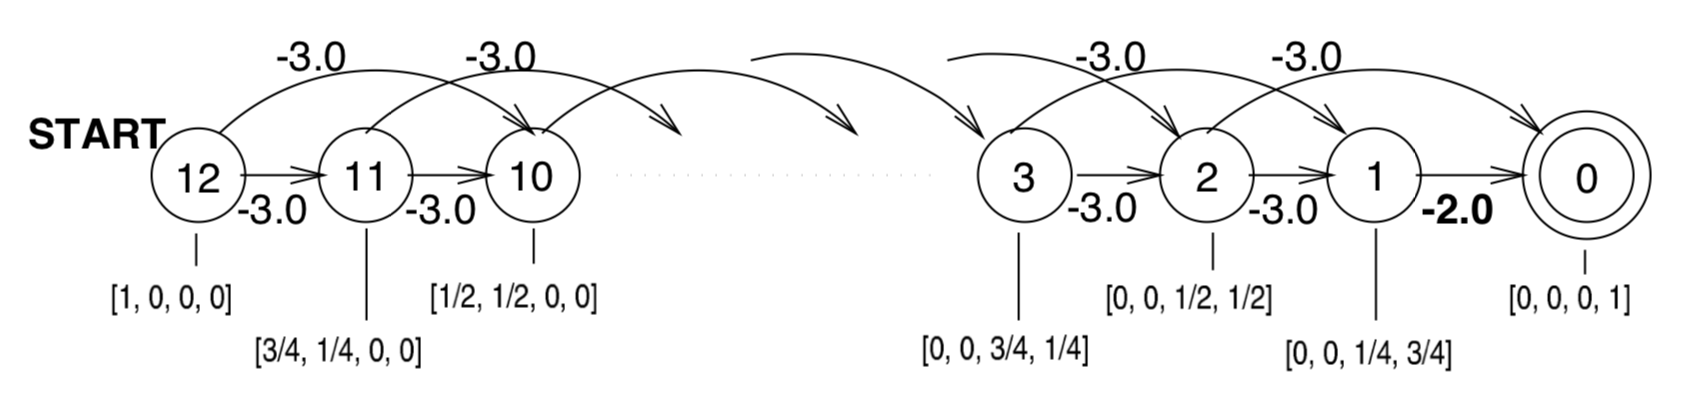
\includegraphics[width=10 cm]{picture/acyclic_MDP}
\caption{An example of acyclic MDP.}
\label{fig:acy_MDP} 
\end{figure}

The acyclic MDP may look like Figure \ref{fig:acy_MDP}. For this case, I give the dynamic programming algorithm to solve this problem. Note that the triple $(s, a, s')$ can be regarded as the edge in the acyclic graph.

\begin{algorithm}[h]
\caption{Dynamic Programming for Acyclic MDP} 
\label{alg::DP_acy} 
\begin{algorithmic}[1]
{
\Require
$s, s'$: state;
$a$: action;
$\gamma$: discount factor;
$A(s)$: the feasible action set of state $s$;
$V(s)$: the optimal value of state $s$;
$R(s)$: the reward of state $s$;
$T(s, a, s')$: the transition from state $s$ to $s'$ by taking action $a$
\Ensure
$V$: the optimal values of all states
\State $V(s_{start})$ = $R(s_{start})$
\State unexplored = $List(S)$    \texttt{//add all states to the \textit{unexplored} list}
\State $s = s_{start}$
\While {unexplored.$isNotEmpty$}
	\State unexplored.$pop$(s)    \texttt{//pop the current state $s$ to avoid repetition}
	\State children\_list = $Successor(s)$    \texttt{//all the reachable state from state $s$}
	\For {$s' \in children\_list$}    \texttt{//select next state}
		\If{$\forall s'' \in Ancestor(s')$, $V(s'')$ is settled}
			\State $s = s'$    \texttt{//move to next calculable state, with all ancestors settled}
			\State \textbf{Break}
		\EndIf
	\EndFor
	\State value\_list $= []$    \texttt{//carry out DP}
	\For {$s' \in Ancestor(s)$}    \texttt{//value iteration}
		\State value\_list.\textit{append}(($a, R(s') + \gamma T(s', a, s)V(s)$)) \texttt{//the triple is used only once}
	\EndFor
	\State $a_{opt}(s), V_{opt}(s) = max$(value\_list)
\EndWhile
}
\end{algorithmic} 
\end{algorithm}

The basic rationale of this DP algorithm is pretty simple by calculating the optimal value of each state one by one. Note that there is a key procedure to ensure all of the ancestor states of the feasible state are settled in that the DP needs all of its ancestors' optimal values. Take the example of Figure \ref{fig:acy_MDP}. After settling the start state 12, we can go to 11 or 10. But one of the ancestor of state 10 is 11 and the value of state 11 is not settled yet, so I have to choose state 11 as the next state to carry out DP. I ensure every $(s', a, s)$ triple is used only once by using a list to record every unexplored state. During the explore of each state $s$, the ancestor state $s'$ is explored only once. As a consequence, the state $s$ and $s'$ are used together only once, thus the $(s', a, s)$ triple is used only once.

\subsection{Problem 2c}









%----------------------------------------------------------------------------------------

\end{spacing}
\end{document}